\section{Optymalizacja przy użyciu pakietu JModelica.org}
\label{sec:opt}

Podstawowym zadaniem wyższego poziomu aplikacji było przeprowadzenie optymalizacji w celu wyznaczenia sterowania czasooptymalnego. Jak wspomniano w sekcji \ref{sub:czesc-wyzsza-wybor}, wybrano do tego celu platformę JModelica.org.

%-------------------------------------------------
\subsection{Opis algorytmu optymalizacji dynamicznej}
\label{sub:opt-alg}
%TODO: opisać algorytm CasADI

Algorytm wykorzystywany do optymalizacji dynamicznej można ogólnie opisać jako bezpośrednią metodę kolokacji. Polega ona na aproksymacji układu równań różniczkowych w dyskretnych chwilach czasu i konstrukcji na tej podstawie zadania programowania nieliniowego, zwykle o rzadkiej strukturze. Jest napisana w języku Python i używa biblioteki CasADi do wyznaczenia wartości pochodnych funkcji oraz oprogramowania IPOPT do obliczenia wynikowego zagadnienia programowania nieliniowego. Można z niej korzystać pod warunkiem, że model matematyczny nie zawiera nieciągłości (za: \cite{JModelicaUserGuide}). W związku z tym, że nieciągłość występuje w rozważanym modelu zbiorników dla zerowego poziomu w trzecim zbiorniku, należało unikać trajektorii zawierających ten punkt.

Programy rozwiązujące problemy NLP wykazują się dużo większą zbieżnością w przypadku, gdy dostarczy się im informacje o pochodnych pierwszego i drugiego rzędu (za: \cite{and+11mod11}). W związku z tym w użytym algorytmie użyto najpierw oprogramowania CasADi, aby ze skompilowanego modelu w języku Modelica wyznaczyć wartości tych pochodnych (w formie jakobianu), a następnie używa się metody elementów skończonych. Dzieli ona wyjściowy przedział czasowy na określoną liczbę przedziałów nazywanych elementami skończonymi i dostarcza aproksymacji nieznanych wartości sterowania i stanów systemu w określonej liczbie punktów kolokacji. Wpływ liczby elementów na jakość rozwiązania jest przedstawiony w sekcji \ref{sub:sym-wer-jmodelica}.
W każdym punkcie kolokacji zastosowano pakiet IPOPT, który rozwiązuje zadanie w postaci danej wzorem \ref{eq:opt-stat} za pomocą metody punktu wewnętrznego. Metoda ta wykorzystuje funkcję graniczną do poruszania się tylko wewnątrz zbioru dopuszczalnego, gdzie metodą Newtona szuka lokalnego minimum.

\begin{equation}\label{eq:opt-stat}
    \min\limits_{x \in [x_{l}, x_{u}]} f(x),~~ g_{l} <= g(x) <= g_{u}
\end{equation}


%-------------------------------------------------
\subsection{Inicjalizacja optymalizacji dynamicznej}
\label{sub:opt-init}

Kluczowym aspektem funkcjonowania algorytmów optymalizacji dynamicznej jest odpowiednie określenie punktu początkowego, czyli początkowej struktury sterowania i wygenerowanej przez nią trajektorii układu. Jest to zagadnienie szeroko opisywane w literaturze, m.in w \cite{Betts98}, \cite{Rao2010}, \cite{Korytowski2015}, \cite{cas+11ifac} oraz \cite{JModelicaUserGuide}.
Początkowo próbowano inicjalizować algorytm stałym sterowaniem, którego wartość jest niezależna od punktów początkowych i końcowych. Niestety, takie podejście okazało się błędne i nie udało się wyznaczyć żadnego sterowania optymalnego.

W związku z tym przyjęto następujący algorytm inicjalizacyjny:
\begin{itemize}
    \item dla każdej z trzech wartości poziomów docelowych wyznacz wartość sterowania ustalonego na podstawie odwrotności wzoru \ref{eq:model-steady-state} danego wzorem \ref{eq:steady-ctrls},
    \begin{equation} \label{eq:steady-ctrls}
    u_{i} = C_{i}h_{i}^{\alpha_{i}}
    \end{equation}
    \item wyznacz wartość średnią z trzech sterowań ustalonych, wyznaczonych w poprzednim kroku według wzoru \ref{eq:steady-ctrl}
    \begin{equation}\label{eq:steady-ctrl}
    u_{r} = \frac{1}{3} \cdot \sum_{i=1}^{3} u_{i}
    \end{equation}
    \item przeprowadź symulację z czasem końcowym podanym jako wartość właściwości \emph{SimulationFinaltime} (opisanej w sekcji \ref{sub:czesc-wyzsza-klasa}),
    \item podaj wyniki uzyskane w symulacji jako trajektorie inicjalizacyjne do algorytmu optymalizacji.
\end{itemize}

Rysunek \ref{fig:initialguess} przedstawia przykładowe sterowanie ustalone i przebiegi zmiennych stanu uzyskane według powyższego algorytmu.

\begin{figure}[tph]
    \centering
    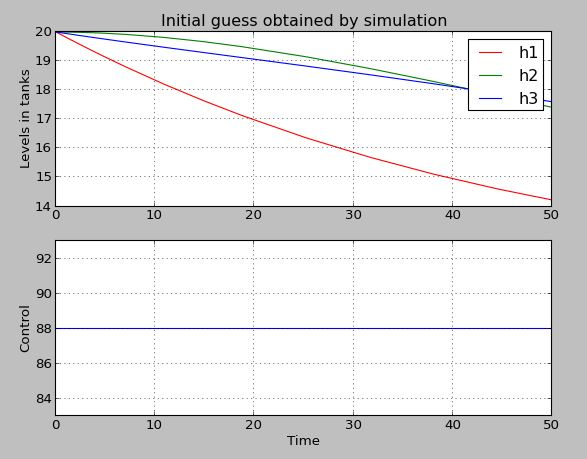
\includegraphics[scale=0.9]{Grafika/initial_guess}
    \caption{Przykładowa trajektoria początkowa dla algorytmu optymalizacji. Źródło: własne.}
    \label{fig:initialguess}
\end{figure}


%-------------------------------------------------
\subsection{Uzyskana postać sterowania}
\label{sub:opt-ctrl-form}
%TODO: opisac heurystyke normalizacji sterowania


%-------------------------------------------------
\subsection{Dokładność wyznaczania rozwiązania}
\label{sub:opt-dokladnosc}
%TODO: opisać wpływ wartości tolerancji IPOPT na rozwiązanie
